\documentclass[11pt,a4paper]{article}
\usepackage[utf8]{inputenc}
\usepackage[T5]{fontenc}
\usepackage{lmodern}
\usepackage[margin=2.2cm]{geometry}
\usepackage{booktabs}
\usepackage{tabularx}
\usepackage{enumitem}
\usepackage{graphicx}
\usepackage{float}
\usepackage{caption}
\usepackage[hidelinks]{hyperref}
\graphicspath{{../figures/}}
\setlist{nosep,leftmargin=1.4em}
\captionsetup{font=small,labelfont=bf}

\title{Flash-Sale Microservices\\[2pt]\large Progress Report, Weeks 1--12}
\author{Vũ Tấn Minh -- 523V0012\\Vũ Đình Kiệt -- 523V0011\\[8pt]
\normalsize Instructor: Mai Văn Mạnh}
\date{23 October 2026}

\begin{document}
\maketitle

\section*{Summary}
The project builds and evaluates a flash-sale order pipeline on .NET~10 and
ABP: an Order Service, an Inventory Service and a Process Worker, with
PostgreSQL, Redis Lua stock reservation, RabbitMQ with a Transactional Outbox
and Inbox, and Nginx. The research question is how this asynchronous design
(C2) compares with a synchronous PostgreSQL baseline (C1), and what load
shedding (C3) and extra Inventory consumers (C4) change.

All of Weeks 1--12 is complete: milestones M1--M5 are ticked with saved
evidence. Week~12 added overload control at three layers and the required AWS
deployment, with one EC2 backend and JMeter on a separate machine, tested in
two live sessions. Weeks 13--15 (pilot, official runs, submission) remain.

\begin{table}[H]
\centering
\small
\begin{tabularx}{\textwidth}{llX}
\toprule
Milestone & Weeks & Status \\
\midrule
M1 Foundation & 1--2 & Done: scope, six-state order model, ERD, local environment \\
M2 Baseline and design & 3--4 & Done: C0 race shown, C1 baseline correct, contracts, test plan \\
M3 Intake and stock workflow & 5--8 & Done: Order API, Outbox, Redis Lua reservation, stock results, validator \\
M4 Recovery and observability & 9--11 & Done: Inbox, retry/DLQ, reconciliation, Worker, metrics and extraction \\
M5 Overload and deployment & 12 & Done: load shedding, Outbox-backlog admission, Terraform/EC2, overload recovery \\
M6--M8 Pilot, official runs, QA & 13--15 & Next \\
\bottomrule
\end{tabularx}
\end{table}

\section{System overview}
A client posts an order to Order Service, which writes the order and an
\texttt{OrderPlaced} Outbox row in one transaction and answers 201
immediately. A publisher sends the event to RabbitMQ with publisher confirms.
Inventory Service reserves one unit atomically in Redis (Lua) and publishes
\texttt{StockReserved} or \texttt{StockRejected}. Order Service and the
Process Worker consume it, and the order moves through the six states of the
brief (Figure~\ref{fig:states}). The Order Service and Inventory Service
consumers have an Inbox, so a redelivered message never takes stock twice; the
Process Worker keeps no state and gives its events fixed message ids, so
Order Service's Inbox drops the repeats. Failed messages are retried a bounded
number of times and then dead-lettered; a reconciliation job re-publishes
orders stuck in \texttt{PendingStock}.

\begin{figure}[H]
\centering
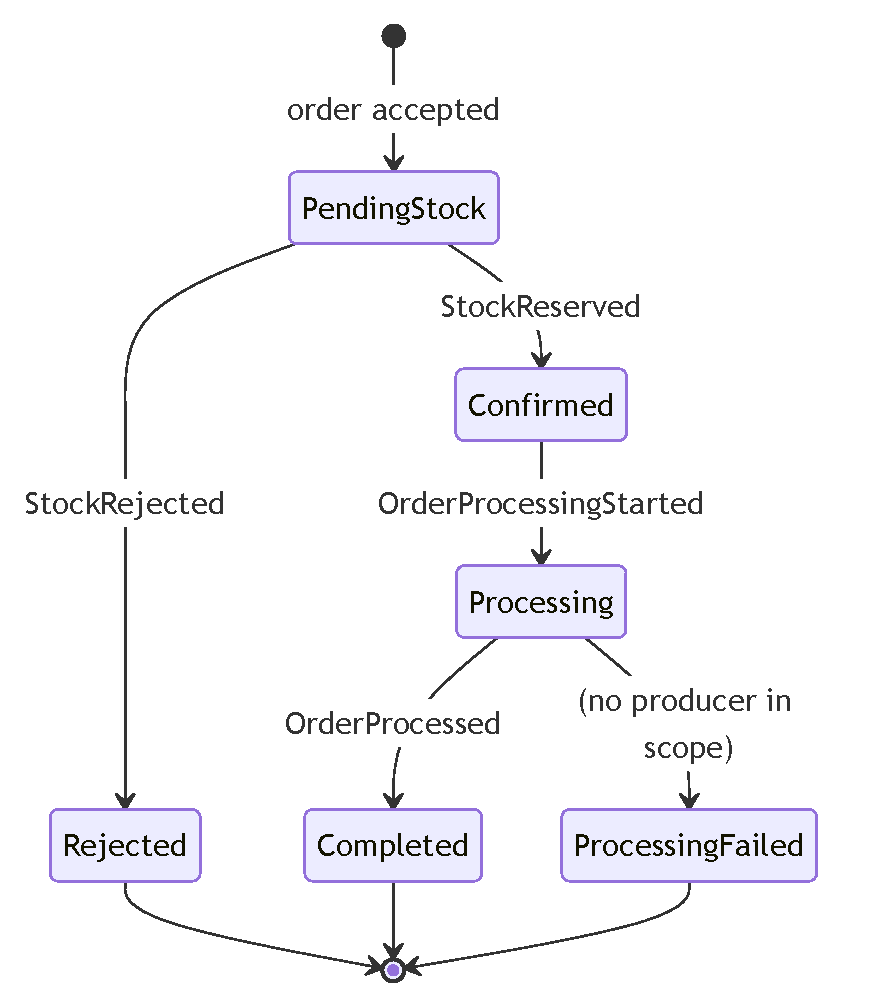
\includegraphics[width=0.52\textwidth]{state-machine}
\caption{Order states. \texttt{ProcessingFailed} is declared but has no
producer, because the Worker is success-only in scope.}
\label{fig:states}
\end{figure}

\section{Weeks 1--11 in brief}
\begin{itemize}
  \item \textbf{Weeks 1--4.} Scope, invariants and protocol were written; the
    local stack and the ERD matched the code; C0 reproduced the race
    condition and C1 never oversold; contracts and a named test plan were
    written, and unsupported claims were removed.
  \item \textbf{Weeks 5--8.} Idempotent order intake (one order per key; a
    retry gets the original); a transactional Outbox with confirmed,
    mandatory publishing; atomic Redis reservation that survives a
    PostgreSQL failure without a second deduction; and a validator that
    reports INCONCLUSIVE instead of PASS when its evidence is incomplete.
  \item \textbf{Weeks 9--11.} Inbox de-duplication under crashes and
    duplicates; bounded retry and per-service dead-letter queues; stuck-order
    reconciliation; the deterministic Process Worker and the
    \texttt{Processing} state; tracing, metrics, a run-time collector and
    metric extraction for the Results chapter.
\end{itemize}

\section{Week 12: overload control and deployment}

\paragraph{Load shedding (C3).} Four limits, all off by default so C2 is
unchanged (Figure~\ref{fig:layers}). Nginx rate-limits new orders (429).
Order Service refuses a new order before any database write (503 with
\texttt{Retry-After}) when its concurrency slots are full, when its Outbox
backlog is full, or, added after the review below, when too many orders are
still unfinished anywhere in the pipeline. RabbitMQ main queues are bounded,
and since every consumer now takes at most 20 unacknowledged messages, the
bound covers real work; a full queue only delays publication through the
Outbox. Order Service never refuses a retry of an accepted order, but Nginx
can still answer 429 before the retry reaches it, so clients retry with
back-off. The validator gained a C3 mode and a check that every accepted
order ends terminal or is listed as outstanding.

\begin{figure}[H]
\centering
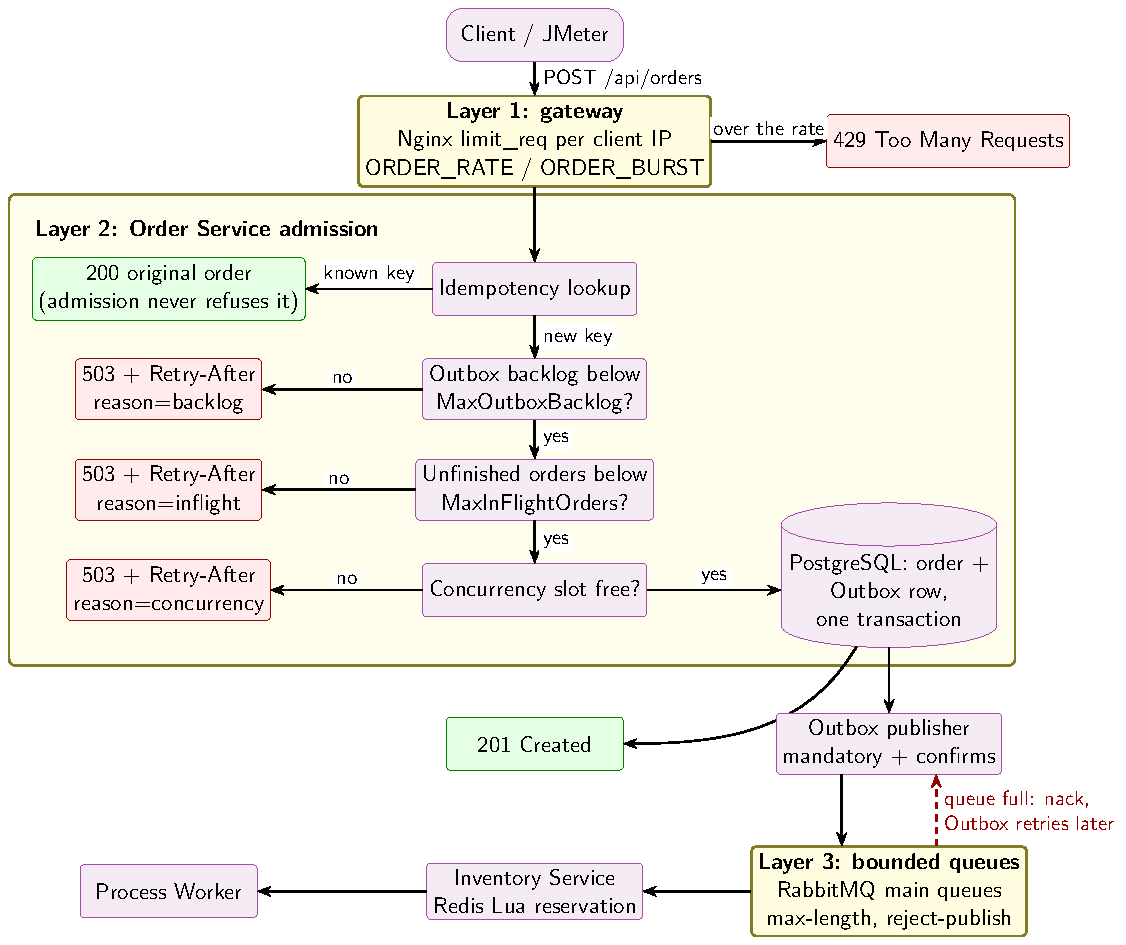
\includegraphics[width=\textwidth]{load-shedding-layers}
\caption{Where each load-shedding layer refuses work.}
\label{fig:layers}
\end{figure}

\paragraph{Overload, drain and recovery.} A three-phase JMeter run (3, 60,
then 3 orders/s) with every limit on. Table~\ref{tab:overload} shows the local
run before and after the review fixes, and the EC2 run, which used the
earlier code. Once all queued work was counted, the earlier local numbers
turned out to hide a backlog behind the Process Worker (about 3.7 orders/s):
Order Service accepted about 13 orders/s during the overload, orders waited
about 40\,s end to end, and the backlog took 105\,s to clear, failing the
60\,s target. With the Worker's queue bounded, it also held back Inventory's
result to Order Service, so orders sat in \texttt{PendingStock} for about
32\,s. With the new in-flight limit, Order Service refuses what the
Worker cannot finish (Figure~\ref{fig:timeline}): fewer orders are accepted
(548 instead of 808), but each one completes in about 6\,s, and the backlog
clears in 7\,s. In every run, refusals matched JMeter, the Nginx log and the
admission metric exactly; none of the sampled refused requests (10 of each
kind) left an order; every accepted order completed with exactly one unit of
stock; and the services recovered without a restart. With every limit
switched off, 3,747 orders got in and the backlog did not drain in time, so
the test does detect missing limits.

\begin{figure}[H]
\centering
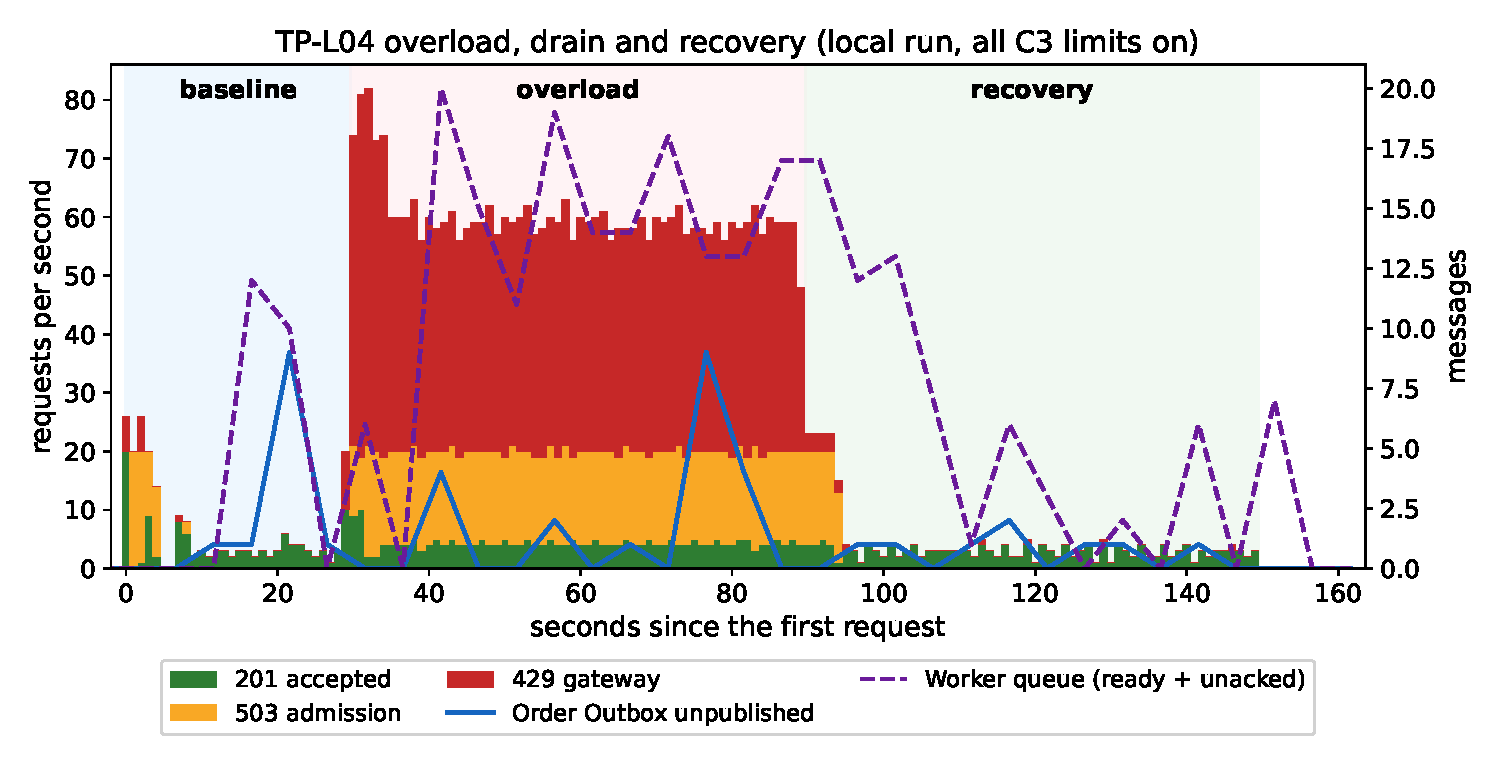
\includegraphics[width=\textwidth]{overload-timeline}
\caption{Local overload run with the in-flight limit, second by second:
accepted (green), admission 503 (orange), gateway 429 (red); the Order Outbox
and the Process Worker queue stay small and clear within seconds.}
\label{fig:timeline}
\end{figure}

\begin{table}[H]
\centering
\footnotesize
\setlength{\tabcolsep}{4pt}
\begin{tabular}{lrrrr}
\toprule
Overload run (pre-pilot limits) & Local 22 Oct & Local 23 Oct & Local 23 Oct & EC2 22 Oct \\
 & (before) & (+ prefetch) & (+ in-flight limit) & (before) \\
\midrule
Order submissions & 3,995 & 4,027 & 4,084 & 4,029 \\
Refused 429 / 503 & 2,390 / 832 & 2,403 / 816 & 2,464 / 1,072 & 2,411 / 720 \\
Accepted, all completed & 773 & 808 & 548 & 898 \\
Accepted to Completed, p50 / p95 & 38 / 64\,s & 40 / 66\,s & 6.1 / 6.8\,s & -- \\
Backlog drain after overload & 3.9\,s\textsuperscript{a} & 105\,s & 6.9\,s & 2.4\,s\textsuperscript{a} \\
Final drain after the last request & 59\,s & 55\,s & 7.1\,s & 48\,s \\
Recovery time\textsuperscript{b} & 7\,s & 5\,s & 7\,s & -- \\
Recovery-phase p95 latency & 63\,ms & 55\,ms & 34\,ms & 19\,ms \\
\bottomrule
\end{tabular}
\caption{One run each; official values come from Weeks 13--14. The in-flight
limit was the database baseline + 30. \textsuperscript{a}The earlier, narrower
measure that missed messages already delivered to the Worker; not comparable
with the other two. \textsuperscript{b}First 10\,s window after the recovery
phase starts with no refusals, no errors, p95 $\le$ 1\,s and at least one
accepted order per second. The EC2 run used the code from before the review;
its raw data was not archived, so it cannot be re-measured.}
\label{tab:overload}
\end{table}

\paragraph{AWS deployment.} Terraform creates two EC2 hosts, a backend
(\texttt{m7i-flex.large}) and a separate JMeter host
(\texttt{c7i-flex.large}), in
\texttt{ap-southeast-2} (Figure~\ref{fig:ec2}). The backend runs the stack in
Docker Compose with pinned images; only Nginx is reachable, and only from the
JMeter host. There is no SSH (AWS Systems Manager is used instead), no NAT,
Elastic IP or load balancer, and a 4-hour self-terminate safety timer. The
owner applies and destroys; the assistant only reads the account and runs
commands on the two tagged hosts. Two sessions passed: only port 80 answered
from the JMeter host, the smoke test ran 44 of 44 requests successfully, and
both sessions were destroyed with nothing left behind.

\begin{figure}[H]
\centering
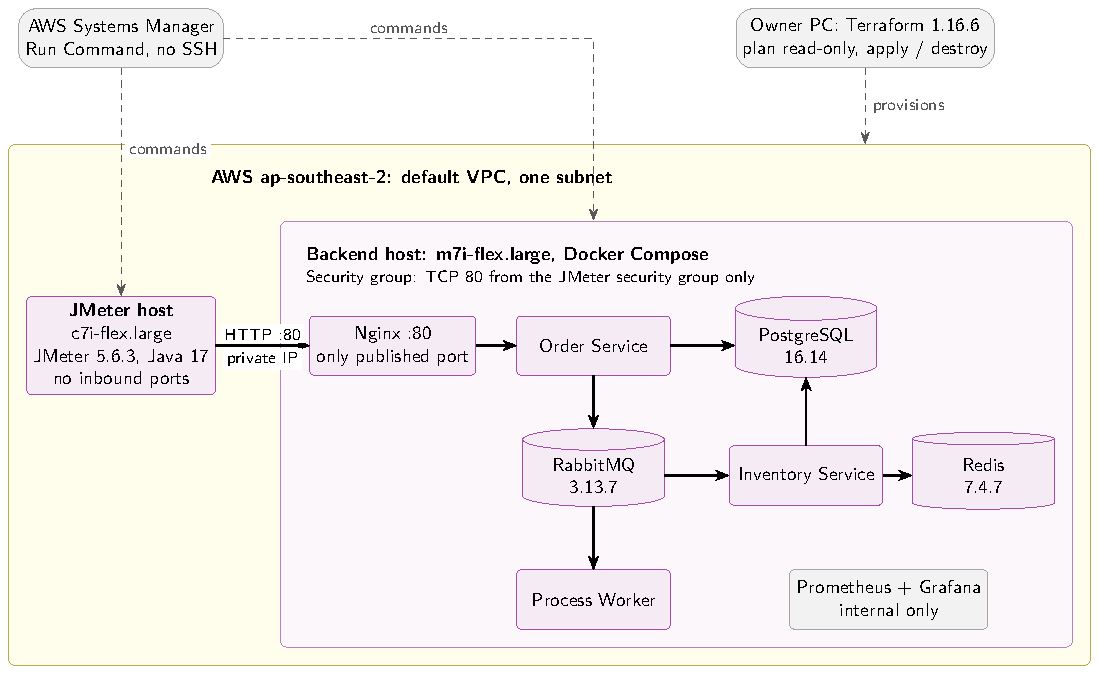
\includegraphics[width=\textwidth]{ec2-deployment}
\caption{The Week 12 EC2 deployment.}
\label{fig:ec2}
\end{figure}

\paragraph{Review findings fixed in Week 12.} Code review and testing
caught, among others:
\begin{itemize}
  \item an Nginx redirect that sent every POST past the rate limit;
  \item a rate-limit bypass through a trailing slash or upper-case path;
  \item a stale Outbox-backlog count that never refused while the broker was
    down;
  \item a missing .NET image tag and image pins older than the tested stack;
  \item fixed development database passwords on EC2;
  \item an Nginx gateway that exposed the admin UI.
\end{itemize}
Each was fixed and re-tested before its box was ticked.

\section{Verification}
Every claim links to a saved log in \texttt{tests/evidence/}. On the final
code, all 18 runtime verifiers pass with no failures
(Figure~\ref{fig:verif}; the counts are read from the logs, not typed in),
along with 98 of 98 unit tests. Each fix below has a test that fails when
the fix is removed. The chart counts checks; it does not rank how strong each
verifier is.

\begin{figure}[H]
\centering
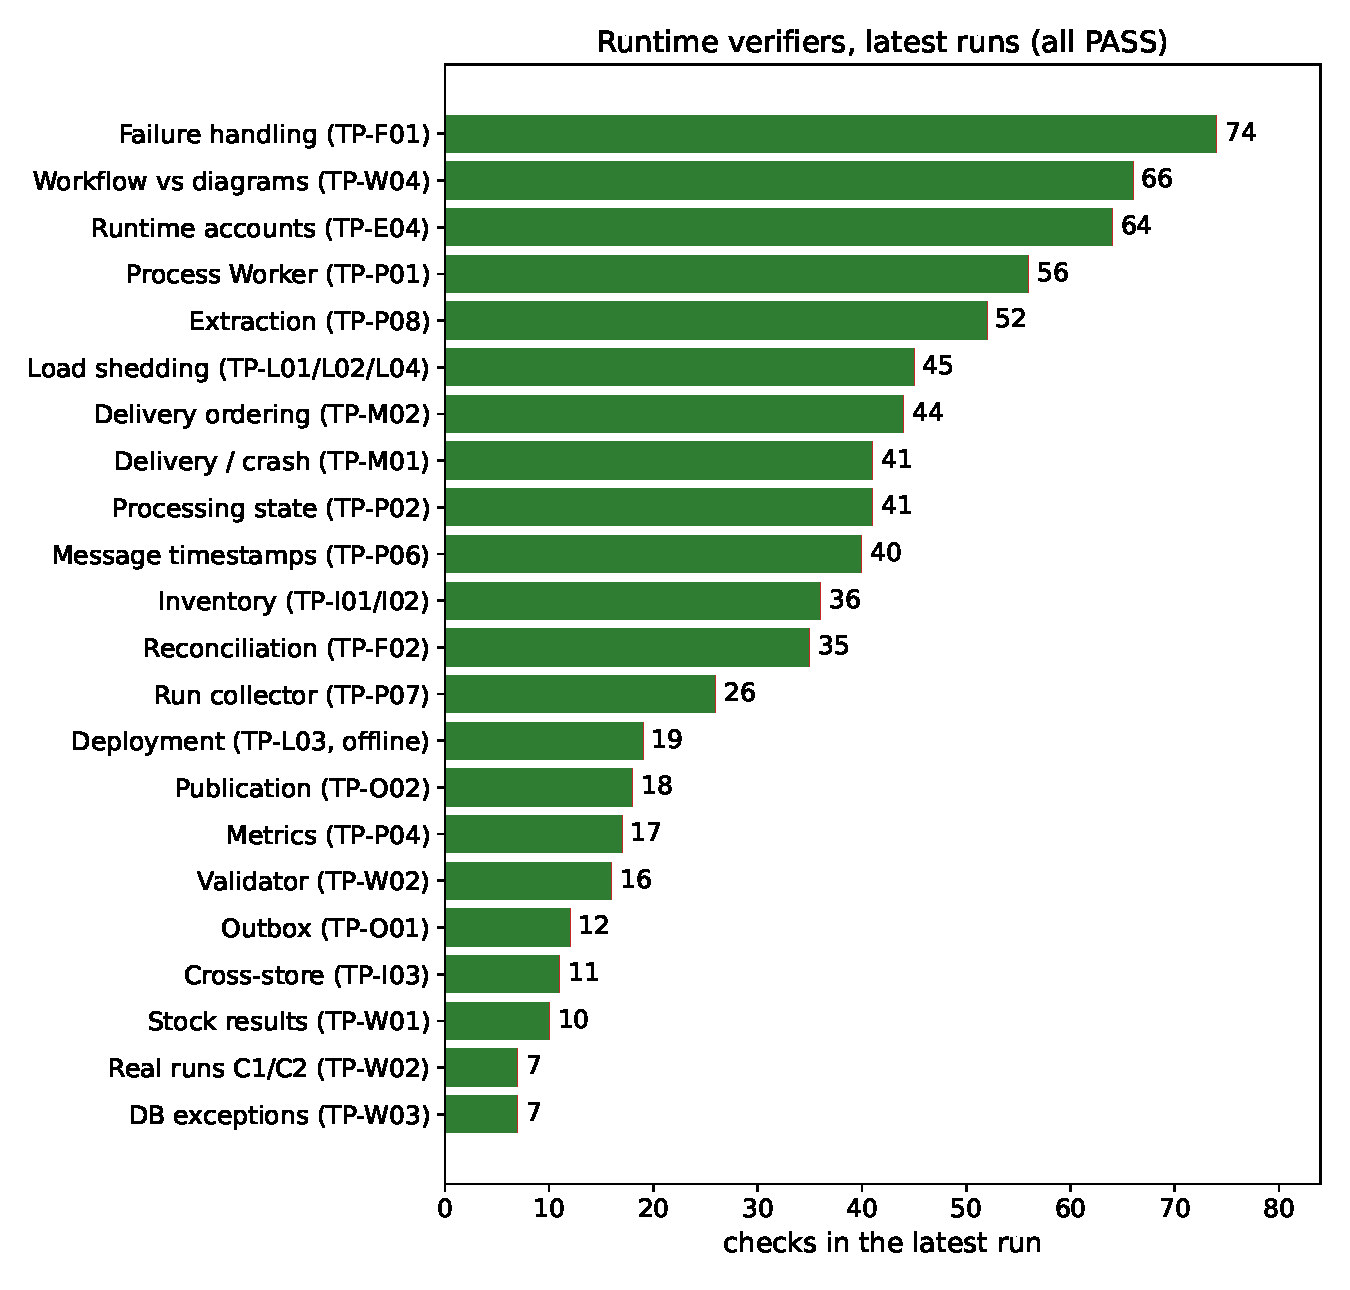
\includegraphics[width=0.92\textwidth]{verification-overview}
\caption{Checks per runtime verifier in its latest run.}
\label{fig:verif}
\end{figure}

\section{External review after Week 12}
An external review graded Weeks 1--12 strictly. We confirmed its findings in
the code or the saved data, fixed them, and re-tested everything:
\begin{itemize}
  \item \textbf{State regression.} A late ``processing started'' event could
    move a \texttt{Completed} order back to \texttt{Processing}. The order's
    state is now a concurrency token; a late event re-reads and is
    acknowledged as stale.
  \item \textbf{Hidden backlog.} No consumer limited its unacknowledged
    messages, so the Worker held its whole backlog outside the queue bound.
    Every consumer now takes at most 20, the backlog measure counts all
    queued work, and the new in-flight limit keeps the backlog small.
  \item \textbf{Measurement.} The metric extractor now counts a run's orders
    by their own keys (773, not 771), stops on any SQL error instead of
    reading it as 0, and counts recovery only when nothing is being refused.
    Publish times are taken when a message is sent, which removed 714
    negative publish-to-decision intervals.
  \item \textbf{Reconciliation} now also recovers orders stuck in
    \texttt{Confirmed} or \texttt{Processing} (lost Worker work).
  \item \textbf{Report wording} that overclaimed was corrected.
\end{itemize}
Still open: the EC2 overload numbers describe the code from before the
review, and all limits are pre-pilot values.

\section{Next steps}
\begin{enumerate}
  \item \textbf{Week 13 pilot and freeze:} pilot C1--C4 (1, 2 and 4 Inventory
    consumers) on EC2, set the load-shedding limits from the pilot (the
    Outbox-backlog bound refused everything on EC2 and needs tuning), make
    the Process Worker's metrics reachable on EC2, and freeze source,
    configuration and the run matrix. Copy every EC2 run's raw data back
    before the stack is destroyed.
  \item \textbf{Week 14:} official repeated runs (3--5 per cell), figures,
    and the complete report; reproduce a validated run from the README by
    13 November 2026.
  \item \textbf{Week 15:} final QA and submission by 21 November 2026.
\end{enumerate}

\end{document}
